\chapter{进程与线程}\label{OS02}

\section{进程实体、PCB 与线程}\label{OS02-process-thread}

进程是程序的一次执行过程及其资源环境，是资源分配和管理的基本单位。进程实体由程序段、数据段和 PCB 构成；PCB 是进程存在和管理的标志，记录标识、状态、调度信息、资源与处理器现场。进程具有动态性、并发性、独立性、异步性和结构性，动态性是最基本特征。

\par\smallskip
{\fontsize{9.3}{12}\selectfont\setlength{\tabcolsep}{2.5pt}\setlength{\LTleft}{0pt}\setlength{\LTright}{0pt}
\begin{longtable}{@{}>{\raggedright\arraybackslash}p{\dimexpr0.29441\linewidth-2\tabcolsep\relax}>{\raggedright\arraybackslash}p{\dimexpr0.70559\linewidth-2\tabcolsep\relax}@{}}
\toprule
对象 & 共享与独有内容 \\

\midrule\endfirsthead\toprule
对象 & 共享与独有内容 \\

\midrule\endhead\bottomrule\endfoot
不同进程 & 各有 PCB 与地址空间；通信共享须按机制建立 \\

同进程线程 & 共享代码、数据、堆、打开文件等进程资源 \\

每条线程 & 独有 TID、PC、寄存器现场、栈、运行状态、优先级等 TCB 信息 \\

\end{longtable}}
\par\smallskip

支持内核级线程时，内核按可调度线程分配处理器；纯用户级线程由线程库调度，内核仍调度其承载实体。同进程线程的栈用于各自调用链，其他线程取得有效地址后仍可能访问它。父子进程各有 PCB、可并发执行；写时复制可暂时共享物理页，逻辑地址空间仍分别管理。

\section{状态转换与进程控制}\label{OS02-states}

\par\smallskip
{\fontsize{9.3}{12}\selectfont\setlength{\tabcolsep}{2.5pt}\setlength{\LTleft}{0pt}\setlength{\LTright}{0pt}
\begin{longtable}{@{}>{\raggedright\arraybackslash}p{\dimexpr0.33594\linewidth-2\tabcolsep\relax}>{\raggedright\arraybackslash}p{\dimexpr0.66406\linewidth-2\tabcolsep\relax}@{}}
\toprule
转换 & 条件 \\

\midrule\endfirsthead\toprule
转换 & 条件 \\

\midrule\endhead\bottomrule\endfoot
就绪 → 运行 & 被调度并获得 CPU \\

运行 → 就绪 & 时间片到期、被抢占、主动让出 CPU 且仍具执行条件 \\

运行 → 阻塞 & 等待 I/O、资源或同步事件 \\

阻塞 → 就绪 & 对应等待条件满足，执行唤醒 \\

\end{longtable}}
\par\smallskip

就绪仅缺 CPU；阻塞还缺事件。单 CPU 同一时刻至多一个相应实体运行。阻塞者须先就绪再运行；就绪者未执行，不能主动发起新的阻塞操作。

\begin{figure}[H]
\centering
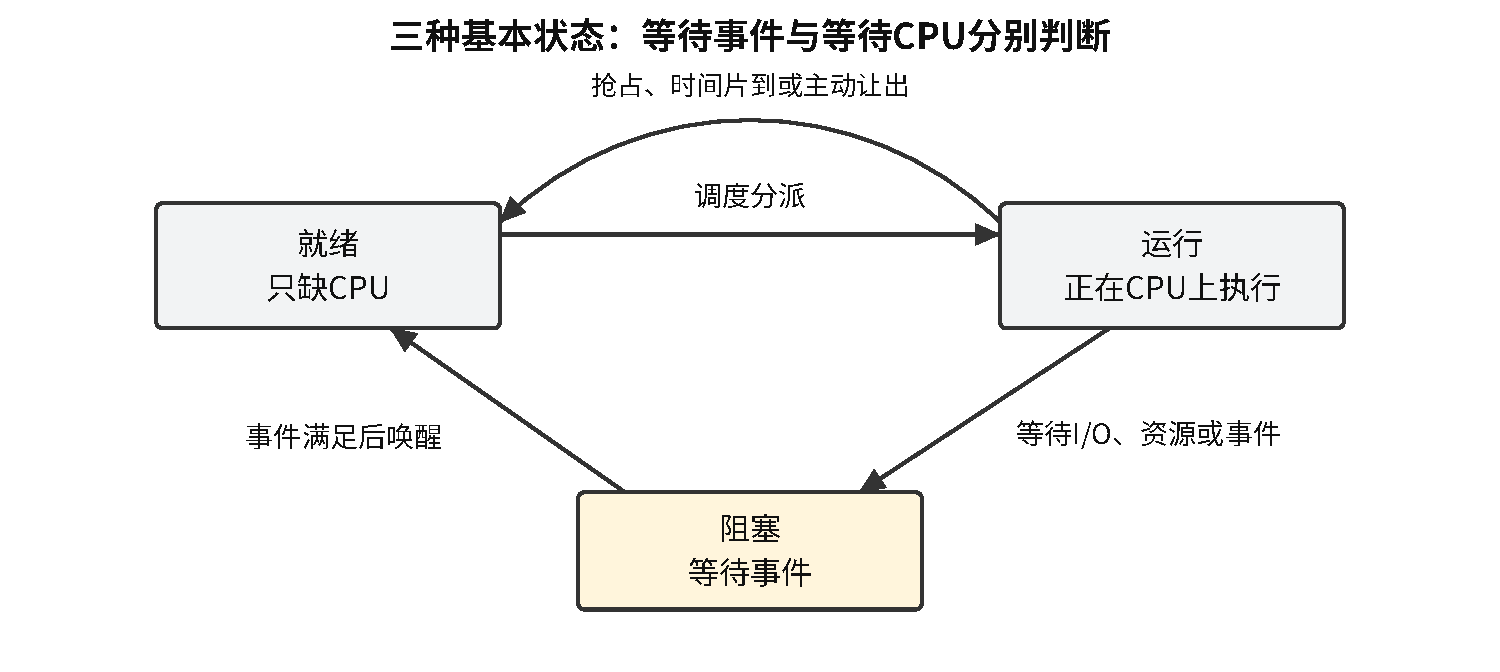
\includegraphics[width=\linewidth,height=108mm,keepaspectratio]{figures/OS_process_states.pdf}
\caption{运行、就绪、阻塞的转换条件}
\end{figure}

七状态模型在创建、就绪、运行、阻塞、终止上增加就绪挂起和阻塞挂起。经典模型的挂起表示映像暂不驻留内存，PCB 继续保留；阻塞挂起者事件满足后转为就绪挂起；激活后分别进入就绪或阻塞。运行者也可被挂起，创建者可按策略进入就绪或就绪挂起。

\par\medskip\Needspace{4\baselineskip}\noindent\hypertarget{OS02-E01}{}\label{OS02-E01}\textbf{例 2-1}\par\nobreak\smallskip

下列由当前线程引起的事件或执行的操作中，可能导致该线程由执行态变为就绪态的是（　）。

A. 键盘输入　　B. 缺页异常　　C. 主动出让 CPU　　D. 执行信号量的 wait() 操作

\par\smallskip
{\fontsize{9.3}{12}\selectfont\setlength{\tabcolsep}{2.5pt}\setlength{\LTleft}{0pt}\setlength{\LTright}{0pt}
\begin{longtable}{@{}>{\raggedright\arraybackslash}p{\dimexpr0.26748\linewidth-2\tabcolsep\relax}>{\raggedright\arraybackslash}p{\dimexpr0.73252\linewidth-2\tabcolsep\relax}@{}}
\toprule
控制原语 & 必须一致更新的内容 \\

\midrule\endfirsthead\toprule
控制原语 & 必须一致更新的内容 \\

\midrule\endhead\bottomrule\endfoot
创建 & 申请标识、PCB 与资源，初始化现场，加入就绪等队列 \\

撤销 & 停止执行、处理通知及等待关系、回收资源与 PCB；子进程政策依系统 \\

阻塞 & 保存现场、改状态、进入对应事件等待队列并调度 \\

唤醒 & 移出等待队列、改为就绪、加入就绪队列 \\

切换 & 保存旧现场、更新状态队列、恢复新现场 \\

\end{longtable}}
\par\smallskip

PCB 可按状态链接成队列，或由索引表定位；阻塞队列可按事件细分。状态字段与队列关系必须原子维护；进程阻塞后的长时间等待允许 CPU 调度其他进程。

\section{用户级、内核级线程与映射}\label{OS02-thread-models}

\par\smallskip
\begin{wideblock}
{\fontsize{9.3}{12}\selectfont\setlength{\tabcolsep}{2.5pt}\setlength{\LTleft}{0pt}\setlength{\LTright}{0pt}
\begin{longtable}{@{}>{\raggedright\arraybackslash}p{\dimexpr0.17399\linewidth-2\tabcolsep\relax}>{\raggedright\arraybackslash}p{\dimexpr0.40879\linewidth-2\tabcolsep\relax}>{\raggedright\arraybackslash}p{\dimexpr0.41722\linewidth-2\tabcolsep\relax}@{}}
\toprule
模型 & 管理与调度 & 阻塞及并行边界 \\

\midrule\endfirsthead\toprule
模型 & 管理与调度 & 阻塞及并行边界 \\

\midrule\endhead\bottomrule\endfoot
多对一 & 用户线程库管理多个 ULT，内核仅见一个承载实体 & 承载实体阻塞会挡住全部；这些线程不能多核并行 \\

一对一 & 每个用户线程对应一个 KLT，由内核分别调度 & 一个阻塞时其他可运行，可多核并行；管理成本较大 \\

多对多 & 用户线程复用若干 KLT，库与内核分层调度 & 并行度受可用 KLT 与 CPU 核数约束 \\

\end{longtable}}
\end{wideblock}
\par\smallskip

纯用户级切换可不进入内核，开销较小。内核级描述管理方式，应用代码仍可在用户态执行。创建、切换开销随实现而变。

\section{进程通信、管道与信号}\label{OS02-ipc}

\par\smallskip
\begin{wideblock}
{\fontsize{9.3}{12}\selectfont\setlength{\tabcolsep}{2.5pt}\setlength{\LTleft}{0pt}\setlength{\LTright}{0pt}
\begin{longtable}{@{}>{\raggedright\arraybackslash}p{\dimexpr0.16296\linewidth-2\tabcolsep\relax}>{\raggedright\arraybackslash}p{\dimexpr0.44628\linewidth-2\tabcolsep\relax}>{\raggedright\arraybackslash}p{\dimexpr0.39076\linewidth-2\tabcolsep\relax}@{}}
\toprule
机制 & 数据或事件的组织 & 使用条件 \\

\midrule\endfirsthead\toprule
机制 & 数据或事件的组织 & 使用条件 \\

\midrule\endhead\bottomrule\endfoot
共享内存 & 多个虚拟映射指向共同物理区，建立后普通访存交换数据 & 共享布局与访问同步由通信方约定 \\

消息传递 & 直接指定进程，或经信箱／端口间接通信 & 发送、接收是否阻塞由接口规定 \\

管道 & 有限容量、顺序消费的数据流；经典无名管道为半双工、常用于亲缘进程 & 双向可用两条管道；命名管道可按名称联系 \\

信号 & 通知事件，可采用默认动作或获准的用户处理程序 & 普通信号可能合并；部分信号不可捕获、忽略或屏蔽 \\

\end{longtable}}
\end{wideblock}
\par\smallskip

共享内存可按规定数据结构组织，也可提供存储区由进程约定布局。管道空时阻塞读、满时阻塞写；有数据即可读，有空间即可写，无须等待整管装满或读空。读出消耗数据，多读者取得不同数据；字节流通常不保留应用记录边界，原子写长度和请求大小按接口。

普通信号位向量模型：\texttt{pending} 记录待处理，\texttt{blocked} 记录暂缓递送，当前可递送集合

\[D=\mathrm{pending}\;\&\;\sim\mathrm{blocked}.\]

屏蔽信号不使整个进程进入阻塞态。递送可发生在返回用户态等适当时机，用户处理程序一般在用户态执行。信号通知、信号量许可、处理器异常分属不同机制；合法缺页可由内核修复而不递送用户信号。

\section{调度层次、时机与指标}\label{OS02-scheduling-metrics}

\par\smallskip
{\fontsize{9.3}{12}\selectfont\setlength{\tabcolsep}{2.5pt}\setlength{\LTleft}{0pt}\setlength{\LTright}{0pt}
\begin{longtable}{@{}>{\raggedright\arraybackslash}p{\dimexpr0.40587\linewidth-2\tabcolsep\relax}>{\raggedright\arraybackslash}p{\dimexpr0.59413\linewidth-2\tabcolsep\relax}@{}}
\toprule
层次 & 选择或管理的对象 \\

\midrule\endfirsthead\toprule
层次 & 选择或管理的对象 \\

\midrule\endhead\bottomrule\endfoot
高级／作业调度 & 后备作业进入内存并取得运行资格 \\

中级／内存调度 & 换出、换入，调节驻留进程数量 \\

低级／进程调度 & 从就绪执行实体中分配 CPU \\

\end{longtable}}
\par\smallskip

结束、主动阻塞或让出 CPU 时须选择可运行者；新到达、唤醒、时钟到期可触发抢占判断。非抢占策略让当前执行者运行到结束或主动放弃；抢占策略可在规定事件点改选。

调度器选择执行者，分派器恢复现场并交付 CPU。一次中断、一次调度条件检查、一次实际上下文切换须分别计数。内核管理队列的原子临界操作期间限制调度；持有普通资源互斥权的进程仍可能被切换。无普通就绪者时运行最低优先级的 idle 路径，保留中断响应能力。

设到达 \(A_i\)、首次运行 \(S_i\)、完成 \(C_i\)、CPU 服务 \(B_i\)，则

\[T_i=C_i-A_i,\quad R_i=S_i-A_i,\quad T_i^{\mathrm w}=T_i/B_i.\]

仅一个 CPU 段、无 I/O、忽略切换成本时，等待 \(W_i=T_i-B_i\)；有 I/O 时还须扣去阻塞时间。各指标逐项计算后取算术平均，平均带权周转通常无法由两项平均数相除得到。吞吐量为完成任务数／观察时长，利用率为设备忙时长／观察时长；切换、空闲与有效计算的统计口径按题设。

\section{调度算法与事件时间线}\label{OS02-scheduling-algorithms}

\par\smallskip
\begin{wideblock}
{\fontsize{9.3}{12}\selectfont\setlength{\tabcolsep}{2.5pt}\setlength{\LTleft}{0pt}\setlength{\LTright}{0pt}
\begin{longtable}{@{}>{\raggedright\arraybackslash}p{\dimexpr0.17495\linewidth-2\tabcolsep\relax}>{\raggedright\arraybackslash}p{\dimexpr0.39120\linewidth-2\tabcolsep\relax}>{\raggedright\arraybackslash}p{\dimexpr0.43386\linewidth-2\tabcolsep\relax}@{}}
\toprule
算法 & 选择规则 & 条件及限制 \\

\midrule\endfirsthead\toprule
算法 & 选择规则 & 条件及限制 \\

\midrule\endhead\bottomrule\endfoot
FCFS & 就绪到达最早者，通常非抢占 & 长任务可使短任务等待较久，产生护航效应 \\

SJF & 当前就绪者中预计服务时间最短，通常非抢占 & 需预测时间；持续短任务可使长任务饥饿 \\

SRTF & 当前就绪者中剩余时间最短，可抢占 & 新到达时比较当前剩余量 \\

HRRN & 最大 \(1+W/B\)，通常非抢占 & 等待提高响应比，兼顾长短任务 \\

优先级 & 当前就绪者中优先级最高 & 数值方向、抢占及同级顺序按题设；老化可缓解饥饿 \\

RR & 就绪队列轮转，至多运行一个时间片 & 用完未结束者回队尾；过大片接近 FCFS，过小增加开销 \\

多级队列 & 任务通常固定所属队列 & 队间固定优先级或时间比例，队内规则分别规定 \\

多级反馈 & 根据运行行为迁移队列，常用逐级加长时间片 & 高层可抢占低层；降级、I/O 返回及剩余片规则按题设 \\

\end{longtable}}
\end{wideblock}
\par\smallskip

时间线只在已到达且就绪者中选择。记录每次事件的当前执行者、剩余量、各队列顺序；同刻到达与片耗尽的入队次序须明确。CPU 总服务量须与题设一致。最小平均等待等最优性结论需同时到达、已知服务、忽略开销等相应模型前提。

\par\medskip\Needspace{4\baselineskip}\noindent\hypertarget{OS02-E02}{}\label{OS02-E02}\textbf{例 2-2}\par\nobreak\smallskip

4 个作业到达系统的时刻和运行时间如下表所示。

\par\smallskip
{\fontsize{9.3}{12}\selectfont\setlength{\tabcolsep}{2.5pt}\setlength{\LTleft}{0pt}\setlength{\LTright}{0pt}
\begin{longtable}{@{}>{\raggedright\arraybackslash}p{\dimexpr0.33333\linewidth-2\tabcolsep\relax}>{\raggedright\arraybackslash}p{\dimexpr0.33333\linewidth-2\tabcolsep\relax}>{\raggedright\arraybackslash}p{\dimexpr0.33333\linewidth-2\tabcolsep\relax}@{}}
\toprule
作业 & 到达时刻 & 运行时间 \\

\midrule\endfirsthead\toprule
作业 & 到达时刻 & 运行时间 \\

\midrule\endhead\bottomrule\endfoot
J1 & 0 & 3 \\

J2 & 1 & 3 \\

J3 & 1 & 2 \\

J4 & 3 & 1 \\

\end{longtable}}
\par\smallskip

系统在 \(t=2\) 时开始作业调度。若分别采用先来先服务和短作业优先调度算法，则选中的作业分别是（　）。

A. J2、J3　　B. J1、J4　　C. J2、J4　　D. J1、J3

\par\medskip\Needspace{4\baselineskip}\noindent\hypertarget{OS02-E03}{}\label{OS02-E03}\textbf{例 2-3}\par\nobreak\smallskip

进程进入就绪队列的时刻、优先级（值越大优先权越高）及 CPU 执行时间如下表所示。

\par\smallskip
{\fontsize{9.3}{12}\selectfont\setlength{\tabcolsep}{2.5pt}\setlength{\LTleft}{0pt}\setlength{\LTright}{0pt}
\begin{longtable}{@{}>{\raggedright\arraybackslash}p{\dimexpr0.24938\linewidth-2\tabcolsep\relax}>{\raggedright\arraybackslash}p{\dimexpr0.24938\linewidth-2\tabcolsep\relax}>{\raggedright\arraybackslash}p{\dimexpr0.24938\linewidth-2\tabcolsep\relax}>{\raggedright\arraybackslash}p{\dimexpr0.25186\linewidth-2\tabcolsep\relax}@{}}
\toprule
进程 & 到达 & 优先级 & CPU 时间 \\

\midrule\endfirsthead\toprule
进程 & 到达 & 优先级 & CPU 时间 \\

\midrule\endhead\bottomrule\endfoot
P1 & 0 ms & 1 & 60 ms \\

P2 & 20 ms & 10 & 42 ms \\

P3 & 30 ms & 100 & 13 ms \\

\end{longtable}}
\par\smallskip

采用基于优先权的抢占式 CPU 调度算法，从 0 ms 开始调度，三个进程的平均周转时间为（　）。

A. 60 ms　　B. 61 ms　　C. 70 ms　　D. 71 ms

\par\medskip\Needspace{4\baselineskip}\noindent\hypertarget{OS02-E04}{}\label{OS02-E04}\textbf{例 2-4}\par\nobreak\smallskip

P0、P1、P2、P3 的到达、优先级（值越小优先权越高）和执行时间如下表所示。采用基于优先权的抢占式进程调度，从 0 ms 开始，到四个进程都运行结束为止，发生进程调度的总次数为（　）。

\par\smallskip
{\fontsize{9.3}{12}\selectfont\setlength{\tabcolsep}{2.5pt}\setlength{\LTleft}{0pt}\setlength{\LTright}{0pt}
\begin{longtable}{@{}>{\raggedright\arraybackslash}p{\dimexpr0.24938\linewidth-2\tabcolsep\relax}>{\raggedright\arraybackslash}p{\dimexpr0.24938\linewidth-2\tabcolsep\relax}>{\raggedright\arraybackslash}p{\dimexpr0.24938\linewidth-2\tabcolsep\relax}>{\raggedright\arraybackslash}p{\dimexpr0.25186\linewidth-2\tabcolsep\relax}@{}}
\toprule
进程 & 到达 & 优先级 & CPU 时间 \\

\midrule\endfirsthead\toprule
进程 & 到达 & 优先级 & CPU 时间 \\

\midrule\endhead\bottomrule\endfoot
P0 & 0 ms & 15 & 100 ms \\

P1 & 10 ms & 20 & 60 ms \\

P2 & 10 ms & 10 & 20 ms \\

P3 & 15 ms & 6 & 10 ms \\

\end{longtable}}
\par\smallskip

A. 4　　B. 5　　C. 6　　D. 7

\par\medskip\Needspace{4\baselineskip}\noindent\hypertarget{OS02-E05}{}\label{OS02-E05}\textbf{例 2-5}\par\nobreak\smallskip

系统采用二级反馈队列调度。Q1 采用时间片轮转，时间片为 10 ms；Q2 采用短进程优先。系统优先调度 Q1，Q1 为空才调度 Q2；新创建进程先进入 Q1，在 Q1 执行一个时间片后仍未结束则转入 Q2。当前两队列为空，系统依次创建 P1、P2 后开始调度，两者需要的 CPU 时间分别为 30 ms、20 ms。平均等待时间为（　）。

A. 25 ms　　B. 20 ms　　C. 15 ms　　D. 10 ms

\par\medskip\Needspace{4\baselineskip}\noindent\hypertarget{OS02-E06}{}\label{OS02-E06}\textbf{例 2-6}\par\nobreak\smallskip

系统有 4 个进程，预计运行时间和到达就绪队列的时刻如下，单位均为时间配额。分别采用可抢占式短进程优先和时间片轮转调度（时间片为 2），求各进程的调度次序与平均周转时间。

\par\smallskip
{\fontsize{9.3}{12}\selectfont\setlength{\tabcolsep}{2.5pt}\setlength{\LTleft}{0pt}\setlength{\LTright}{0pt}
\begin{longtable}{@{}>{\raggedright\arraybackslash}p{\dimexpr0.31010\linewidth-2\tabcolsep\relax}>{\raggedright\arraybackslash}p{\dimexpr0.31010\linewidth-2\tabcolsep\relax}>{\raggedright\arraybackslash}p{\dimexpr0.37980\linewidth-2\tabcolsep\relax}@{}}
\toprule
进程 & 到达时刻 & 预计运行时间 \\

\midrule\endfirsthead\toprule
进程 & 到达时刻 & 预计运行时间 \\

\midrule\endhead\bottomrule\endfoot
P1 & 0 & 8 \\

P2 & 1 & 4 \\

P3 & 2 & 9 \\

P4 & 3 & 5 \\

\end{longtable}}
\par\smallskip

\par\medskip\Needspace{4\baselineskip}\noindent\hypertarget{OS02-E07}{}\label{OS02-E07}\textbf{例 2-7}\par\nobreak\smallskip

某进程调度程序采用基于优先数（priority）的调度策略，即选择优先数最小的进程运行。进程创建时由用户指定一个 nice 作为静态优先数。为了动态调整优先数，引入运行时间 cpuTime 和等待时间 waitTime，初值均为 0。进程处于执行态时，cpuTime 定时加 1，且 waitTime 置 0；进程处于就绪态时，cpuTime 置 0，waitTime 定时加 1。请回答下列问题。

（1）若调度程序只将 nice 的值作为进程的优先数，即 priority=nice，则可能会出现饥饿现象，为什么？

（2）使用 nice、cpuTime 和 waitTime 设计一种动态优先数计算方法，以避免产生饥饿现象，并说明 waitTime 的作用。

\section{多处理机与上下文切换}\label{OS02-context}

公共就绪队列便于分担负载，访问须互斥；每核私有队列降低争用，需迁移平衡负载。推迁移由系统负载监测程序推动，拉迁移由空闲或较空闲 CPU 的调度程序取任务。软亲和性倾向留在原 CPU，硬亲和性限制允许 CPU 集合；迁移收益须扣除缓存、TLB 局部性和同步成本。SMT 的逻辑处理器共享核内部分执行资源。

上下文包含 PC、PSW、通用寄存器、栈等恢复状态；例如 \texttt{x+\allowbreak{}+\allowbreak{}} 在寄存器已加一、尚未写回时被切换，必须保存该寄存器与下一指令位置。模式切换只改变执行权限，可仍执行原进程。

同进程线程切换需换线程现场，通常保留进程页表与文件资源；跨进程还需建立新地址空间环境。TLB 是否清空取决于地址空间标识等机制，普通数据 Cache 无须因进程切换一律全部清空。

\section{临界区与互斥要求}\label{OS02-critical-section}

临界资源在同一时期只许一个进程使用；临界区是访问该资源的代码段，进入区申请、退出区释放。多个进程访问同一资源可有多段相关临界区。同步规定操作先后，互斥限制访问重叠。高级语言 \texttt{x=\allowbreak{}x+\allowbreak{}1} 的读、加、写可被交错，单核也可能丢失更新。

\par\smallskip
{\fontsize{9.3}{12}\selectfont\setlength{\tabcolsep}{2.5pt}\setlength{\LTleft}{0pt}\setlength{\LTright}{0pt}
\begin{longtable}{@{}>{\raggedright\arraybackslash}p{\dimexpr0.26748\linewidth-2\tabcolsep\relax}>{\raggedright\arraybackslash}p{\dimexpr0.73252\linewidth-2\tabcolsep\relax}@{}}
\toprule
要求 & 准确含义 \\

\midrule\endfirsthead\toprule
要求 & 准确含义 \\

\midrule\endhead\bottomrule\endfoot
空闲让进 & 临界区空闲，申请者有进入机会 \\

忙则等待 & 已有进入者时，其他相关申请者等待 \\

有限等待 & 请求后被其他进入者越过次数有有限上界；需执行机会和有限临界区等前提 \\

让权等待 & 无法进入时阻塞，让出 CPU \\

\end{longtable}}
\par\smallskip

\par\medskip\Needspace{4\baselineskip}\noindent\hypertarget{OS02-E08}{}\label{OS02-E08}\textbf{例 2-8}\par\nobreak\smallskip

进程 A 和进程 B 通过共享缓冲区协作完成数据处理，进程 A 负责产生数据并放入缓冲区，进程 B 从缓冲区读数据并输出。进程 A 和进程 B 之间的制约关系是（　）。

A. 互斥关系　　B. 同步关系　　C. 互斥和同步关系　　D. 无制约关系

\section{软件互斥、原子指令与锁}\label{OS02-locks}

双进程软件模型假定共享单次读写原子、顺序一致。\texttt{i=\allowbreak{}0,\allowbreak{}1}，\texttt{j=\allowbreak{}1-i}，\texttt{flag} 初值均为假。

\par\smallskip
\begin{wideblock}
{\fontsize{9.3}{12}\selectfont\setlength{\tabcolsep}{2.5pt}\setlength{\LTleft}{0pt}\setlength{\LTright}{0pt}
\begin{longtable}{@{}>{\raggedright\arraybackslash}p{\dimexpr0.20350\linewidth-2\tabcolsep\relax}>{\raggedright\arraybackslash}p{\dimexpr0.39808\linewidth-2\tabcolsep\relax}>{\raggedright\arraybackslash}p{\dimexpr0.39842\linewidth-2\tabcolsep\relax}@{}}
\toprule
方案 & 进入／退出规则 & 失效原因 \\

\midrule\endfirsthead\toprule
方案 & 进入／退出规则 & 失效原因 \\

\midrule\endhead\bottomrule\endfoot
单标志 & 等 \texttt{turn==i}；退出置 \texttt{turn=j} & 强制交替，对方不申请时也可能阻挡，违背空闲让进 \\

双标志先检查 & 等 \texttt{!flag{[}j{]}} 后置 \texttt{flag{[}i{]}=true}；退出清自身标志 & 双方可先检查通过再置真，破坏互斥 \\

双标志后检查 & 先置自身真，再等对方假；退出清自身标志 & 双方都置真后互等，临界区空闲仍无法进入 \\

\end{longtable}}
\end{wideblock}
\par\smallskip

Peterson 同时表达意愿与让步：

\par\smallskip\noindent\begin{minipage}{\linewidth}
\begin{codeblock}[language={}]
flag[i] = true;
turn = j;
while (flag[j] && turn == j) { }
临界区;
flag[i] = false;
\end{codeblock}
\end{minipage}\par\smallskip

在上述内存模型与持续调度、有限临界区条件下，Peterson 满足互斥和有限等待；循环检查仍占 CPU。实际机器需原子变量和适当内存序。

\par\smallskip\noindent\begin{minipage}{\linewidth}
\begin{codeblock}[language={}]
// TestAndSet 原子返回旧值并置真；lock 初值 false
while (TestAndSet(lock)) { }
临界区;
lock = false;

// Swap 原子交换；key 为进程私有
key = true;
while (key) Swap(lock, key);
临界区;
lock = false;
\end{codeblock}
\end{minipage}\par\smallskip

TS／Swap 的检查与占用整体原子；普通赋值展开式须额外原子化。这些自旋实现保证互斥，公平和有限等待还需另设机制。持锁很短且持有者可继续执行时可减少睡眠切换开销；较长等待适合阻塞锁。单核自旋须允许持锁者获得执行机会。本 CPU 关中断仅保护合适的单处理器内核路径，普通用户程序无权执行，亦无法阻挡其他 CPU。

\section{信号量的数值语义与前驱同步}\label{OS02-semaphores}

本章 \texttt{P=\allowbreak{}wait}、\texttt{V=\allowbreak{}signal}，均采用记录型信号量；队列公平性须额外声明。P、V 的计数更新、判断与入队／唤醒须原子化。

\par\smallskip\noindent\begin{minipage}{\linewidth}
\begin{codeblock}[language={}]
P(S): S.value--;
      if (S.value < 0) 入队并阻塞;
      // 唤醒后本次 P 返回，不再减 1
V(S): S.value++;
      if (S.value <= 0) 移出一个等待者并置为就绪;
\end{codeblock}
\end{minipage}\par\smallskip

\texttt{value>\allowbreak{}0} 为未分配许可数；\texttt{value=\allowbreak{}0} 为无剩余许可且无该量等待者；\texttt{value<\allowbreak{}0} 的绝对值为等待者数。P 减后为 0 可继续；V 加后为 0 仍须唤醒。V 不因缺资源而阻塞，唤醒后仍等 CPU。整型信号量在 \texttt{S<\allowbreak{}=\allowbreak{}0} 时忙等、再原子减一，通常无负值，需与记录型数值规则分开。

互斥量初值 1；容量 \(n\)、初存 \(k\) 件时 \texttt{empty=\allowbreak{}n-k,\allowbreak{} full=\allowbreak{}k}；未完成通知初值 0。信号量初值来自初态，P 与对应 V 可分属不同进程，通常无互斥锁 API 的持有者限制。

\par\medskip\Needspace{4\baselineskip}\noindent\hypertarget{OS02-E09}{}\label{OS02-E09}\textbf{例 2-9}\par\nobreak\smallskip

用 P、V 操作实现进程同步，信号量的初值为（　）。

A. \ensuremath{-}1　　B. 0　　C. 1　　D. 由用户确定

前驱边 \(A\to B\) 可用初值 0 的 \texttt{done}：前进程 \texttt{A;\allowbreak{} V(\allowbreak{}done)\allowbreak{}}，后进程 \texttt{P(\allowbreak{}done)\allowbreak{};\allowbreak{} B}。同线程顺序已保证的边无需重复通知；多路汇合须等待每路完成，分叉须分别发布许可。通知放在前操作完成后、后操作开始前，避免增加题设未要求的先后约束。

\par\medskip\Needspace{4\baselineskip}\noindent\hypertarget{OS02-E10}{}\label{OS02-E10}\textbf{例 2-10}\par\nobreak\smallskip

某进程的两个线程 T1 和 T2 并发执行 A、B、C、D、E 和 F 共 6 个操作，其中 T1 执行 A、E 和 F，T2 执行 B、C 和 D。题46图表示上述 6 个操作的执行顺序所必须满足的约束：C 在 A 和 B 完成后执行，D 和 E 在 C 完成后执行，F 在 E 完成后执行。请使用信号量的 wait()、signal() 操作描述 T1 和 T2 之间的同步关系，并说明所用信号量的作用及其初值。

\begin{figure}[H]
\centering
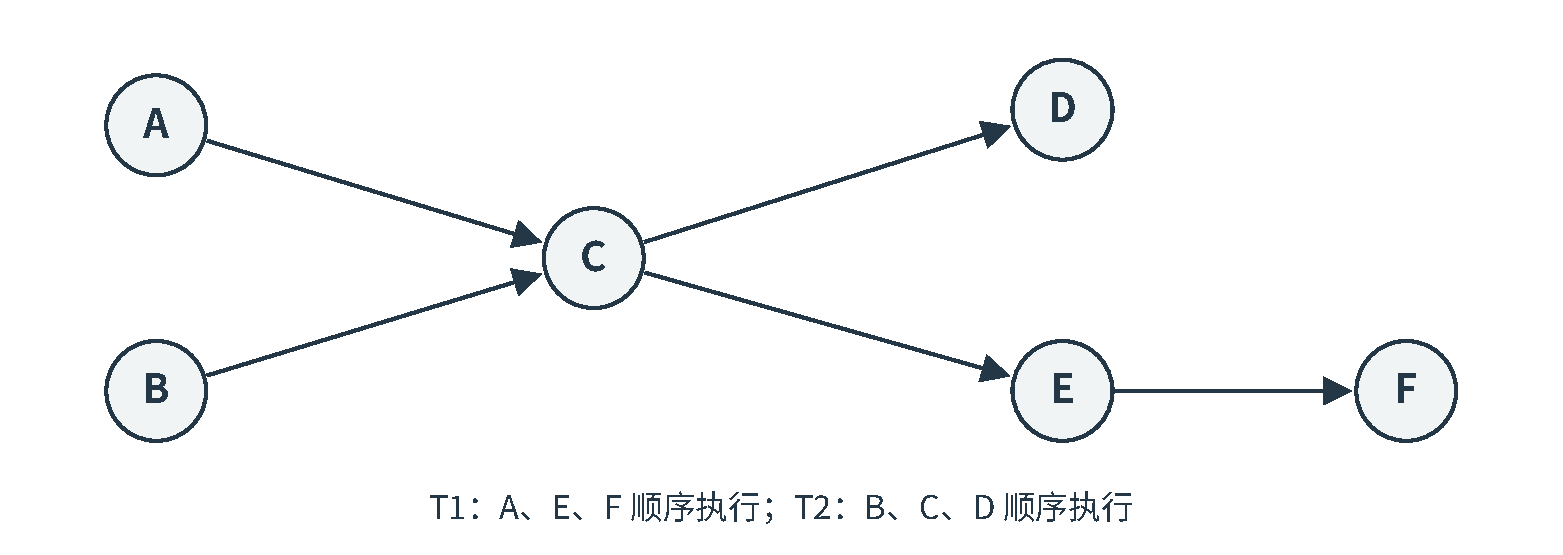
\includegraphics[width=\linewidth,height=108mm,keepaspectratio]{figures/F03_precedence_2022.pdf}
\caption{原题前驱图；图下文字标明题干给出的线程归属}
\end{figure}

\section{生产者与消费者}\label{OS02-buffer}

容量 \(n>0\)，初始为空，生产和消费可反复进行，每次放取一件；共享缓冲及指针须互斥。局部生产、使用产品放在锁外。

\par\smallskip\noindent\begin{minipage}{\linewidth}
\begin{codeblock}[language={}]
semaphore empty=n, full=0, mutex=1;
producer: while (true) {
    x=produce();
    P(empty); P(mutex);
    put(x);
    V(mutex); V(full);
}
consumer: while (true) {
    P(full); P(mutex);
    x=get();
    V(mutex); V(empty);
    consume(x);
}
\end{codeblock}
\end{minipage}\par\smallskip

本模板先取得容量／产品许可，再取得缓冲锁。空缓冲时若先持 \texttt{mutex} 再等 \texttt{full}，生产者无法放入，形成死锁。放入完成后两次 V 可交换，条件是消费者仍须持同一锁访问；这种可交换性依赖具体代码。

许可可能已预留或尚未发布，记录型值还可为负；逐指令执行时 \texttt{empty+\allowbreak{}full=\allowbreak{}n} 与``full 等于实存产品数''均不恒成立。静止且无预留、未发布或等待者时，才能直接对应物理数量。

\par\medskip\Needspace{4\baselineskip}\noindent\hypertarget{OS02-E11}{}\label{OS02-E11}\textbf{例 2-11}\par\nobreak\smallskip

计算机系统中的进程之间往往需要相互协作以完成一个任务。在某网络系统中，缓冲区 B 用于存放一个数据分组，对 B 的操作有 C1、C2 和 C3。C1 将一个数据分组写入 B 中，C2 从 B 中读出一个数据分组，C3 对 B 中的数据分组进行修改。要求 B 为空时才能执行 C1，B 非空时才能执行 C2 和 C3。

（1）假设进程 P1 和 P2 均需要执行 C1，实现 C1 的代码是否为临界区？为什么？（2分）

（2）假设 B 初始为空，进程 P1 执行 C1 一次，进程 P2 执行 C2 一次。请定义尽可能少的信号量，并用 wait()、signal() 操作描述进程 P1 和 P2 之间的同步或互斥关系，说明所用信号量的作用及其初值。（3分）

（3）假设 B 初始不为空，进程 P1 和 P2 各执行 C3 一次。请定义尽可能少的信号量，并用 wait()、signal() 操作描述进程 P1 和 P2 之间的同步或互斥关系，说明所用信号量的作用及其初值。（3分）

分类产品分别设置可消费许可，共用空位和缓冲锁；连续取 \(k\) 件需消费者批锁覆盖整批，单件缓冲锁只覆盖放取，等待产品时保留生产者补货通路。

\par\medskip\Needspace{4\baselineskip}\noindent\hypertarget{OS02-E12}{}\label{OS02-E12}\textbf{例 2-12}\par\nobreak\smallskip

三个进程 P1、P2、P3 互斥使用一个包含 N（N\textgreater0）个单元的缓冲区。P1 每次用 produce() 生成一个正整数并用 put() 送入缓冲区某一空单元中；P2 每次用 getodd() 从该缓冲区中取出一个奇数并用 countodd() 统计奇数个数；P3 每次用 geteven() 从该缓冲区中取出一个偶数并用 counteven() 统计偶数个数。请用信号量机制实现这三个进程的同步与互斥活动，并说明所定义信号量的含义（要求用伪代码描述）。

\par\medskip\Needspace{4\baselineskip}\noindent\hypertarget{OS02-E13}{}\label{OS02-E13}\textbf{例 2-13}\par\nobreak\smallskip

系统中有多个生产者进程和多个消费者进程，共享一个能存放 1000 件产品的环形缓冲区（初始为空）。当缓冲区未满时，生产者进程可以放入其生产的一件产品，否则等待；当缓冲区未空时，消费者进程可以从缓冲区取走一件产品，否则等待。要求一个消费者进程从缓冲区连续取出 10 件产品后，其他消费者进程才可以取产品。请使用信号量 P、V（或 wait()、signal()）操作实现进程间的互斥与同步，要求写出完整的过程，并说明所用信号量的含义和初值。

\section{单盘水果模型}\label{OS02-fruit}

盘子容量 1，初始空；父亲放苹果、母亲放橘子，女儿取苹果、儿子取橘子：

\par\smallskip\noindent\begin{minipage}{\linewidth}
\begin{codeblock}[language={}]
semaphore plate=1, apple=0, orange=0;
father:   while (true) { 准备苹果; P(plate); 放苹果; V(apple); }
mother:   while (true) { 准备橘子; P(plate); 放橘子; V(orange); }
daughter: while (true) { P(apple); 取苹果; V(plate); 吃苹果; }
son:      while (true) { P(orange); 取橘子; V(plate); 吃橘子; }
\end{codeblock}
\end{minipage}\par\smallskip

该容量及交接规则使访问权始终由一个活动持有，同步兼顾盘子互斥。容量增加后，多个生产者可同时取得空位，共享结构还需 \texttt{mutex}；在实际放取动作周围加锁。

\section{读者与写者}\label{OS02-readers}

多个读者可并发读；写者与读者、写者之间互斥。\texttt{count} 记录已登记且未退出的读者，首读者为全组申请 \texttt{rw}，末读者归还，\texttt{cm} 保护计数及首末判断。

\par\smallskip\noindent\begin{minipage}{\linewidth}
\begin{codeblock}[language={}]
semaphore rw=1, cm=1;
int count=0;
reader() {
    P(cm);
    if (count==0) P(rw);
    count++;
    V(cm);
    读文件;
    P(cm);
    count--;
    if (count==0) V(rw);
    V(cm);
}
writer() { P(rw); 写文件; V(rw); }
\end{codeblock}
\end{minipage}\par\smallskip

检查首末与计数修改必须在同一临界区。首读者持 \texttt{cm} 等 \texttt{rw} 时 \texttt{count=\allowbreak{}0}，无旧读者退出依赖 \texttt{cm}，写者释放也无需 \texttt{cm}。本方案读者优先，连续读者可使写者饥饿。

加入入口 \texttt{gate=\allowbreak{}1}：读者在上述登记入口前 \texttt{P(\allowbreak{}gate)\allowbreak{}}、登记后 \texttt{V(\allowbreak{}gate)\allowbreak{}}；写者 \texttt{P(\allowbreak{}gate)\allowbreak{};\allowbreak{} P(\allowbreak{}rw)\allowbreak{};\allowbreak{} 写;\allowbreak{} V(\allowbreak{}rw)\allowbreak{};\allowbreak{} V(\allowbreak{}gate)\allowbreak{}}，读者退出保持原样。写者取得 gate 后阻止新读者登记，旧读者可退出；FIFO 等公平排队、持续调度及有限读写共同支持无饥饿结论，普通信号量本身无此保证。

\section{哲学家进餐}\label{OS02-philosophers}

五人 \(P_i\) 需同时持有 \(C_i\) 与 \(C_{(i+1)\bmod5}\)，各筷子初值 1。全员先取同侧会形成五人各持一根的等待环。限制最多四人进入申请到释放区间：

\par\smallskip\noindent\begin{minipage}{\linewidth}
\begin{codeblock}[language={}]
semaphore room=4, C[5]={1,1,1,1,1};
philosopher(i) {
    while (true) {
        思考;
        P(room); P(C[i]); P(C[(i+1)%5]);
        吃饭;
        V(C[(i+1)%5]); V(C[i]); V(room);
    }
}
\end{codeblock}
\end{minipage}\par\smallskip

四人是申请人数上限，五根筷子最多支持两人同时进餐。其他无环方案：全局按资源编号从小到大申请；用额外互斥量串行化拿两根的过程，拿齐后释放该量，吃完直接归还筷子。所有方案的无饥饿仍需公平条件；各人独立先左后右无法形成全局递增次序。

\section{管程与条件变量}\label{OS02-monitor}

管程封装共享数据、操作及初始化，同一时刻至多一个进程在其中执行，由语言或运行系统保证入口互斥。条件变量管理等待队列，布尔条件由共享状态表示。执行 \texttt{x.\allowbreak{}wait(\allowbreak{})\allowbreak{}} 即入队阻塞并释放管程；\texttt{x.\allowbreak{}signal(\allowbreak{})\allowbreak{}} 通知一个等待者，无人等待时不积累许可。信号量 V 则会留下计数。

\par\medskip\Needspace{4\baselineskip}\noindent\hypertarget{OS02-E14}{}\label{OS02-E14}\textbf{例 2-14}\par\nobreak\smallskip

若 x 是管程内的条件变量，则当进程执行 x.wait() 时所做的工作是（　）。

A. 实现对变量 x 的互斥访问

B. 唤醒一个在 x 上阻塞的进程

C. 根据 x 的值判断该进程是否进入阻塞态

D. 阻塞该进程，并将之插入 x 的阻塞队列中

Hoare 语义可立即把管程交给被通知者；Mesa 语义允许通知者继续，等待者以后重新竞争。Mesa／POSIX 式等待应使用 \texttt{while}：

\par\smallskip\noindent\begin{minipage}{\linewidth}
\begin{codeblock}[language={}]
put(x) {
    lock(m);
    while (count==n) wait(notFull,m);
    插入x; count++;
    signal(notEmpty); unlock(m);
}
get() {
    lock(m);
    while (count==0) wait(notEmpty,m);
    x=取出; count--;
    signal(notFull); unlock(m);
    return x;
}
\end{codeblock}
\end{minipage}\par\smallskip

\texttt{wait} 原子释放锁并入队，返回前重新取得锁；重检处理竞争与可能的虚假唤醒。拆开``解锁、入队''会丢失中间通知。Java 同步实例方法锁定相应对象，静态同步方法锁定类对象；多个实例的锁通常分别存在。

\section{死锁条件、资源图与安全性}\label{OS02-deadlock}

以下讨论可重复使用资源，完成时归还；最大需求可信、可满足后可有限完成。死锁是一组进程各等组内才能产生的事件而无法自行推进；饥饿是个别进程长期得不到服务、其他进程仍可推进；死循环是执行路径持续重复。非重入锁可发生单进程自我死锁。

\par\smallskip
{\fontsize{9.3}{12}\selectfont\setlength{\tabcolsep}{2.5pt}\setlength{\LTleft}{0pt}\setlength{\LTright}{0pt}
\begin{longtable}{@{}>{\raggedright\arraybackslash}p{\dimexpr0.40454\linewidth-2\tabcolsep\relax}>{\raggedright\arraybackslash}p{\dimexpr0.59546\linewidth-2\tabcolsep\relax}@{}}
\toprule
死锁必要条件 & 内容 \\

\midrule\endfirsthead\toprule
死锁必要条件 & 内容 \\

\midrule\endhead\bottomrule\endfoot
互斥 & 实例同一时刻只给一个使用者 \\

占有并等待 & 保持已有资源，再等新增资源 \\

不可剥夺 & 使用中的资源不能被任意收回 \\

循环等待 & 存在首尾相接的资源等待链 \\

\end{longtable}}
\par\smallskip

资源分配图中，进程指向资源为请求边，资源实例指向进程为分配边。无环可排除此模型的死锁；有环且相关资源每类单实例时足以判死锁，多实例时须化简。

安全序列保证每个进程的最大剩余需求可由当时可用量及前者归还量满足。安全表示存在至少一条完整序列；序列可不唯一，也无须强制按其执行。死锁必不安全，不安全可能尚未死锁。

\Needspace{8\baselineskip}

\section{死锁预防、避免与解除}\label{OS02-deadlock-strategies}

\par\smallskip
\begin{wideblock}
{\fontsize{9.3}{12}\selectfont\setlength{\tabcolsep}{2.5pt}\setlength{\LTleft}{0pt}\setlength{\LTright}{0pt}
\begin{longtable}{@{}>{\raggedright\arraybackslash}p{\dimexpr0.20494\linewidth-2\tabcolsep\relax}>{\raggedright\arraybackslash}p{\dimexpr0.40010\linewidth-2\tabcolsep\relax}>{\raggedright\arraybackslash}p{\dimexpr0.39497\linewidth-2\tabcolsep\relax}@{}}
\toprule
策略 & 实施方法 & 条件或代价 \\

\midrule\endfirsthead\toprule
策略 & 实施方法 & 条件或代价 \\

\midrule\endhead\bottomrule\endfoot
预防互斥条件 & 可共享资源改按共享方式组织；SPOOLing 提供逻辑打印服务 & 物理打印仍串行，固有互斥语义须保留 \\

预防占有并等待 & 一次申请全部，或申请失败先释放已有资源 & 需知需求、可能降低利用率 \\

允许剥夺 & 保存恢复资源状态并回滚 & 适合可恢复资源，纸上输出难撤回 \\

预防循环等待 & 统一编号，严格递增申请 & 所有参与者须遵循同一全局次序 \\

避免 & 每次拟分配后检查安全性 & 需最大需求等未来信息，可能推迟现有量足够的请求 \\

检测及解除 & 允许进入死锁，检测后终止、剥夺或回滚 & 考虑已做工作、恢复成本、优先级；反复同一牺牲者可饥饿 \\

\end{longtable}}
\end{wideblock}
\par\smallskip

\par\medskip\Needspace{4\baselineskip}\noindent\hypertarget{OS02-E15}{}\label{OS02-E15}\textbf{例 2-15}\par\nobreak\smallskip

若系统 S1 采用死锁避免方法，S2 采用死锁检测方法。下列叙述中，正确的是（　）。

\ensuremath{\mathrm{I}}. S1 会限制用户申请资源的顺序，而 S2 不会

\ensuremath{\mathrm{II}}. S1 需要进程运行所需的资源总量信息，而 S2 不需要

\ensuremath{\mathrm{III}}. S1 不会给可能导致死锁的进程分配资源，而 S2 会

A. 仅\ensuremath{\mathrm{I}}、\ensuremath{\mathrm{II}}　　B. 仅\ensuremath{\mathrm{II}}、\ensuremath{\mathrm{III}}　　C. 仅\ensuremath{\mathrm{I}}、\ensuremath{\mathrm{III}}　　D. \ensuremath{\mathrm{I}}、\ensuremath{\mathrm{II}}、\ensuremath{\mathrm{III}}

仅降低死锁者优先级无法使其释放资源。预防改变请求规则，避免依据当前状态和最大需求，检测依据当前等待请求。

\section{银行家算法}\label{OS02-banker}

向量按同类资源逐项比较。\texttt{Need=\allowbreak{}Max-Allocation}，\texttt{Available} 为当前未分配量；始终满足总资源守恒。

\par\smallskip\noindent\begin{minipage}{\linewidth}
\begin{codeblock}[language={}]
Work=Available; Finish[0..n-1]=false;
while 存在 i 满足 !Finish[i] && Need[i]<=Work:
    Work += Allocation[i];
    Finish[i]=true;
全部标记：安全；仍有未标记且无可选者：不安全。
\end{codeblock}
\end{minipage}\par\smallskip

模拟中借出的 Need 随完成归还相抵，净增为原 Allocation。检查新请求 \(Q_i\)：{\SNsymbolfont ①} \(Q_i\le Need_i\)；{\SNsymbolfont ②} \(Q_i\le Available\)；{\SNsymbolfont ③}试减 Available、试增 Allocation、试减 Need，完整执行安全检查，安全则提交，否则回滚并等待。

\par\medskip\Needspace{4\baselineskip}\noindent\hypertarget{OS02-E16}{}\label{OS02-E16}\textbf{例 2-16}\par\nobreak\smallskip

某时刻进程的资源使用情况如下表所示，可用资源向量为 \((0,2,1)\)。

\par\smallskip
{\fontsize{9.3}{12}\selectfont\setlength{\tabcolsep}{2.5pt}\setlength{\LTleft}{0pt}\setlength{\LTright}{0pt}
\begin{longtable}{@{}>{\raggedright\arraybackslash}p{\dimexpr0.23351\linewidth-2\tabcolsep\relax}>{\raggedright\arraybackslash}p{\dimexpr0.37435\linewidth-2\tabcolsep\relax}>{\raggedright\arraybackslash}p{\dimexpr0.39214\linewidth-2\tabcolsep\relax}@{}}
\toprule
进程 & 已分配 \((R_1,R_2,R_3)\) & 尚需分配 \((R_1,R_2,R_3)\) \\

\midrule\endfirsthead\toprule
进程 & 已分配 \((R_1,R_2,R_3)\) & 尚需分配 \((R_1,R_2,R_3)\) \\

\midrule\endhead\bottomrule\endfoot
P1 & (2,0,0) & (0,0,1) \\

P2 & (1,2,0) & (1,3,2) \\

P3 & (0,1,1) & (1,3,1) \\

P4 & (0,0,1) & (2,0,0) \\

\end{longtable}}
\par\smallskip

此时的安全序列是（　）。

A. P1、P2、P3、P4　　B. P1、P3、P2、P4

C. P1、P4、P3、P2　　D. 不存在

\par\medskip\Needspace{4\baselineskip}\noindent\hypertarget{OS02-E17}{}\label{OS02-E17}\textbf{例 2-17}\par\nobreak\smallskip

系统有三类资源 A、B、C 和五个进程，某时刻分配如下。若系统安全，则可用资源向量 \((x,y,z)\) 可能是哪些？

\par\smallskip
{\fontsize{9.3}{12}\selectfont\setlength{\tabcolsep}{2.5pt}\setlength{\LTleft}{0pt}\setlength{\LTright}{0pt}
\begin{longtable}{@{}>{\raggedright\arraybackslash}p{\dimexpr0.31845\linewidth-2\tabcolsep\relax}>{\raggedright\arraybackslash}p{\dimexpr0.36309\linewidth-2\tabcolsep\relax}>{\raggedright\arraybackslash}p{\dimexpr0.31845\linewidth-2\tabcolsep\relax}@{}}
\toprule
进程 & Allocation & Max \\

\midrule\endfirsthead\toprule
进程 & Allocation & Max \\

\midrule\endhead\bottomrule\endfoot
P0 & (0,0,3) & (0,0,4) \\

P1 & (1,0,0) & (1,7,5) \\

P2 & (1,3,5) & (2,3,5) \\

P3 & (0,0,2) & (0,6,4) \\

P4 & (0,0,1) & (0,6,5) \\

\end{longtable}}
\par\smallskip

\ensuremath{\mathrm{I}}. (1,4,0)　\ensuremath{\mathrm{II}}. (0,6,2)　\ensuremath{\mathrm{III}}. (1,1,1)　\ensuremath{\mathrm{IV}}. (0,4,7)

A. \ensuremath{\mathrm{I}}、\ensuremath{\mathrm{II}}、\ensuremath{\mathrm{IV}}　　B. \ensuremath{\mathrm{I}}、\ensuremath{\mathrm{II}}　　C. 仅\ensuremath{\mathrm{I}}　　D. \ensuremath{\mathrm{I}}、\ensuremath{\mathrm{III}}

单资源模型总量 100，B、A、T 的 Max 为 70、40、50，Allocation 为 20、10、30，可用 40。给 B 再分 30 后可用 10、Need 为 20、30、20，无人可先完成，应推迟；独立从原态给 A 再分 20 后可用 20、Need 为 50、10、20，可取 T\ensuremath{\to}B\ensuremath{\to}A，Work 为 20\ensuremath{\to}50\ensuremath{\to}70\ensuremath{\to}100。

若 \(n\) 个进程每个最多需 \(k\ge1\) 个同类资源，最坏全员各持 \(k-1\) 个仍未满足；总量

\[m\ge n(k-1)+1\]

足以保证任意分配顺序下至少一人可拿齐并完成。它属于任意分配的总量保证；银行家可通过推迟不安全请求在更少资源下安全运行。

\section{多实例资源的死锁检测}\label{OS02-detection}

检测用当前未满足 \texttt{Request}，避免用未来最大 \texttt{Need}。设 \texttt{Work=\allowbreak{}Available}，通常先将 Allocation 全零者标记完成；反复选择未标记且 \texttt{Request[\allowbreak{}i]\allowbreak{}<\allowbreak{}=\allowbreak{}Work} 者，令 \texttt{Work+\allowbreak{}=\allowbreak{}Allocation[\allowbreak{}i]\allowbreak{}} 并标记。最终持有资源且无法化简者构成死锁核心；无持有量的等待者也可能受其影响，集合范围按题用定义。

设 \(R_1\) 共3、\(R_2\) 共2：P1 持 \((2,0)\)，P2 持 \((1,1)\) 并请求 \((1,0)\)。若 P1 请求 \((0,1)\)，初始 Work=\((0,1)\)，可先 P1 后 P2 完成；若另一 \(R_2\) 由无请求的 P3 持有，P1 请求 \((0,2)\)，P3 归还后 Work 仅 \((0,1)\)，P1、P2 仍无法化简。
